\subsection{Física de la barba}
\label{sec:fisica}

En el modo en vivo, la barba larga se simula con física (\archivo{compositing/beard_physics.py}).

\textbf{Modelo.} Cada hebra es una cadena de cuatro partículas, y hay una hebra por cada 30 píxeles de la región (hasta 2600):
\begin{itemize}
  \item la raíz se guarda en coordenadas baricéntricas de la malla de referencia, así que sigue a la piel en cada cuadro;
  \item la pose de reposo crece en la dirección del pelo y gira con la cabeza;
  \item el largo depende de cuánto está la raíz por debajo de la boca;
  \item las raíces del labio superior crecen hacia los costados, para que no cuelguen sobre los dientes.
\end{itemize}

\textbf{Integración.} En cada cuadro se dan cuatro subpasos de longitud $h=\Delta t/4$ con Verlet amortiguado \cite{verlet1967}:
\begin{align}
  v &= 0{,}86\,(x-x_{\text{prev}}), & x &\leftarrow x+v+g\,h^2, & x &\leftarrow x+k_i\,(x_{\text{reposo}}-x),
\end{align}
con $g=2{,}2\,w$~px/s² y una rigidez $k_i=[0;\,0{,}34;\,0{,}22;\,0{,}13]$ que baja hacia la punta: la base sigue a la cara y la punta tiene inercia. Después, dos iteraciones de restricción de distancia (PBD \cite{jakobsen2001,muller2007}) mantienen el largo de cada tramo. Por eso la hebra se balancea como un péndulo y no se estira. La raíz se interpola entre el cuadro anterior y el actual para que no salte.

\textbf{Render.} Cada hebra se suaviza con un corte de esquinas de Chaikin \cite{chaikin1974}, de 4 a 8 puntos. Cada tramo se dibuja como una gaussiana 2D alargada, con $\sigma$ a lo largo igual a medio tramo y de 0{,}5 a 0{,}75~px a lo ancho. Las gaussianas se acumulan sin ordenar, con densidad $A=\sum o_iG_i$ y cobertura $\alpha=1-e^{-A}$, como en la ley de Beer--Lambert, de modo que muchos pelos superpuestos saturan suavemente. Unos 2000 tramos cuestan unos 10~ms, vectorizados sobre parches de $13\times13$.

En una secuencia con vaivén y un tirón brusco, el retraso de las puntas llega a entre 8 y 12~px y se recupera solo. La correlación entre la velocidad de la cabeza y el retraso es de 0{,}78 a 0{,}82 (figura~\ref{fig:fisica}).

\begin{figure}[ht]
  \centering
  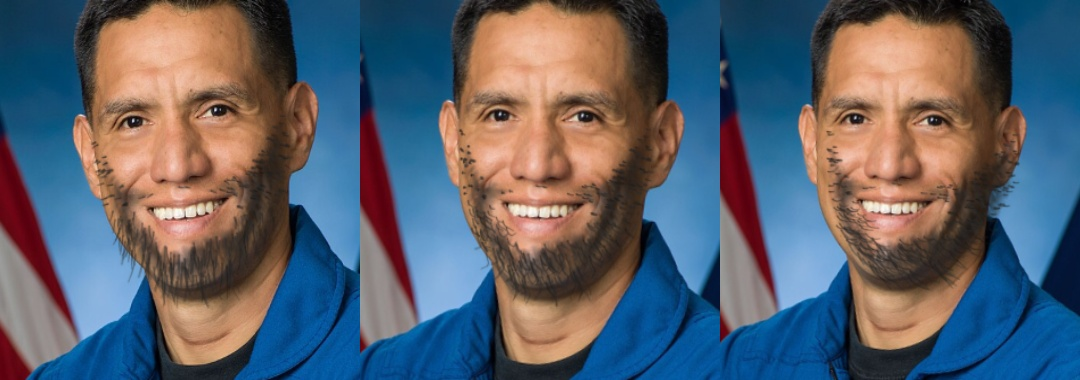
\includegraphics[width=0.85\linewidth]{fisica.jpg}
  \caption{Barba con física: en reposo y durante un movimiento rápido de la cabeza. Las puntas se atrasan y luego vuelven.}
  \label{fig:fisica}
\end{figure}

\subsection{Gaussianas 2D: ``¿Cuántas gaussianas eres?''}
\label{sec:gauss2d}

\archivo{splatting/gaussian_image.py} reconstruye un retrato con $N$ gaussianas 2D, al estilo de GaussianImage \cite{zhang2024}, sin bibliotecas de diferenciación automática.

\textbf{Representación.} Cada gaussiana tiene un centro $\mu_i$, un peso RGB $c_i$ y el factor de Cholesky de la inversa de su covarianza, $L=\begin{psmallmatrix}l_1&0\\l_2&l_3\end{psmallmatrix}$. Con $\Sigma^{-1}=LL^\top$, la covarianza es siempre definida positiva. Con $u=l_1d_x+l_2d_y$ y $v=l_3d_y$:
\begin{equation}
  G_i(x)=\exp\!\big(-\tfrac12(u^2+v^2)\big),\qquad C(x)=\sum_i c_i\,G_i(x).
\end{equation}

\textbf{Optimización.} Se minimiza el error cuadrático medio contra la imagen, usando gradientes analíticos:
\begin{itemize}
  \item respecto de la forma: $\partial q/\partial l_1=2u\,d_x$, $\partial q/\partial l_2=2u\,d_y$ y $\partial q/\partial l_3=2v\,d_y$;
  \item respecto del centro: $\partial q/\partial\mu_x=-2u\,l_1$ y $\partial q/\partial\mu_y=-2u\,l_2-2v\,l_3$.
\end{itemize}
Los parámetros se actualizan con Adam \cite{kingma2015} escrito a mano, en 110 a 160 iteraciones.

\textbf{Detalles de implementación.}
\begin{itemize}
  \item La inicialización coloca más gaussianas donde hay bordes: muestrea con probabilidad proporcional a $0{,}35+|\nabla I|$.
  \item Cada gaussiana se evalúa solo en un parche de radio $\lceil2{,}5\,\sigma_{\max}\rceil$, y los parches se agrupan por radio. Así no hay bucles por gaussiana.
  \item La acumulación usa \texttt{np.bincount}. Una etapa pasó de 10--21~s a 1--4~s.
\end{itemize}

La interfaz lo convierte en un juego: el retrato aparece con 20, 60, 200, 600 y 2000 gaussianas, y hay que reconocer la cara lo antes posible (figura~\ref{fig:gauss2d}).

\begin{figure}[ht]
  \centering
  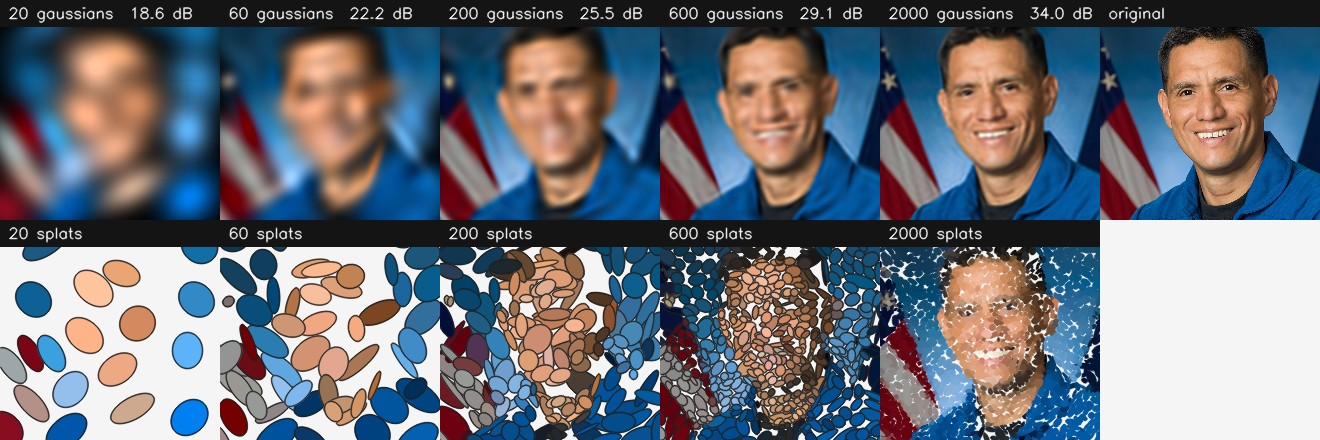
\includegraphics[width=\linewidth]{gaussianas2d.jpg}
  \caption{Retrato reconstruido con 20, 60, 200, 600 y 2000 gaussianas 2D junto al original (arriba), y cada gaussiana dibujada como una elipse (abajo).}
  \label{fig:gauss2d}
\end{figure}

\subsection{Espejo 3D con \emph{Gaussian Splatting}}
\label{sec:espejo}

El espejo convierte una foto en una cabeza de unas 100\,000 gaussianas 3D que se puede girar. Implementa, desde cero, el paso de \emph{render} de 3DGS \cite{kerbl2023}. Las gaussianas no se entrenan desde varias vistas: se construyen a partir de una sola foto y de la malla 3D de MediaPipe.

\textbf{Construcción} (\archivo{splatting/head3d.py}).
\begin{enumerate}
  \item La malla de 478 puntos se triangula con el Delaunay propio en $(x,y)$ y se eleva a 3D con la profundidad estimada.
  \item \textbf{Cara}: cada triángulo recibe gaussianas en proporción a su área 3D (no a la proyectada), con muestreo estratificado. Cada gaussiana es un disco tangente, $\Sigma=R\operatorname{diag}(s^2,s^2,(0{,}4s)^2)R^\top$, donde $R$ es el marco del triángulo. Su color se lee de la foto con interpolación bilineal.
  \item \textbf{Barba}: cada hebra son tres gaussianas alargadas que crecen hacia afuera y hacia abajo desde raíces ancladas con coordenadas baricéntricas.
  \item \textbf{Resto de la foto} (pelo, orejas, fondo): un relieve cuya profundidad se acerca a la del contorno de la cara más cercano, con caída exponencial.
\end{enumerate}

\textbf{Visor} (\archivo{frontend/js/splat3d.js}, WebGL2). Para cada gaussiana:
\begin{itemize}
  \item el \emph{vertex shader} proyecta la covarianza con EWA, $\Sigma_{2D}=JW\Sigma W^\top J^\top+0{,}3\,I$ \cite{zwicker2001}, calcula autovalores y autovectores en forma cerrada y dibuja un cuadrilátero orientado de $\pm3\sigma$;
  \item el \emph{fragment shader} evalúa $\alpha=a\,e^{-r^2/2}$.
\end{itemize}
Las gaussianas se ordenan de atrás hacia adelante con un \emph{counting sort} de 16 bits, en tiempo $O(N)$, y se mezclan con \texttt{SRC\_ALPHA, ONE\_MINUS\_SRC\_ALPHA}. La opción ``Ver cada gaussiana'' achica la huella para mostrar la técnica (figura~\ref{fig:espejo}).

\textbf{Exportación.} Se exporta al formato \texttt{.ply} de 3DGS, compatible con visores externos:
\begin{itemize}
  \item la covarianza se descompone en escala y cuaternión;
  \item el color pasa a armónicos esféricos de grado 0, $f=(c-0{,}5)/0{,}2821$;
  \item la opacidad pasa a \emph{logit}.
\end{itemize}

\begin{figure}[ht]
  \centering
  \begin{subfigure}{0.32\linewidth}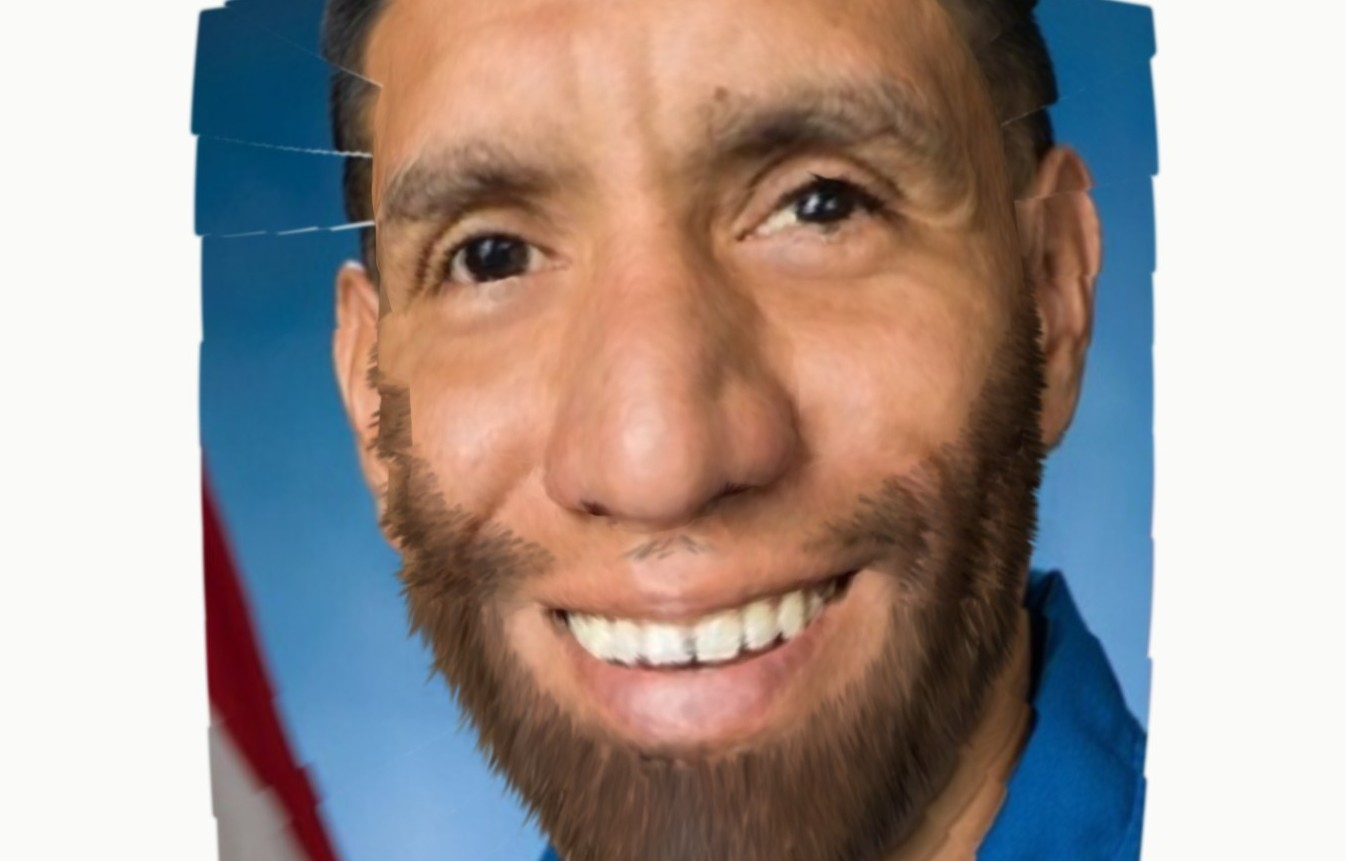
\includegraphics[width=\linewidth]{espejo3d_frente.jpg}\caption{Frente}\end{subfigure}\hfill
  \begin{subfigure}{0.32\linewidth}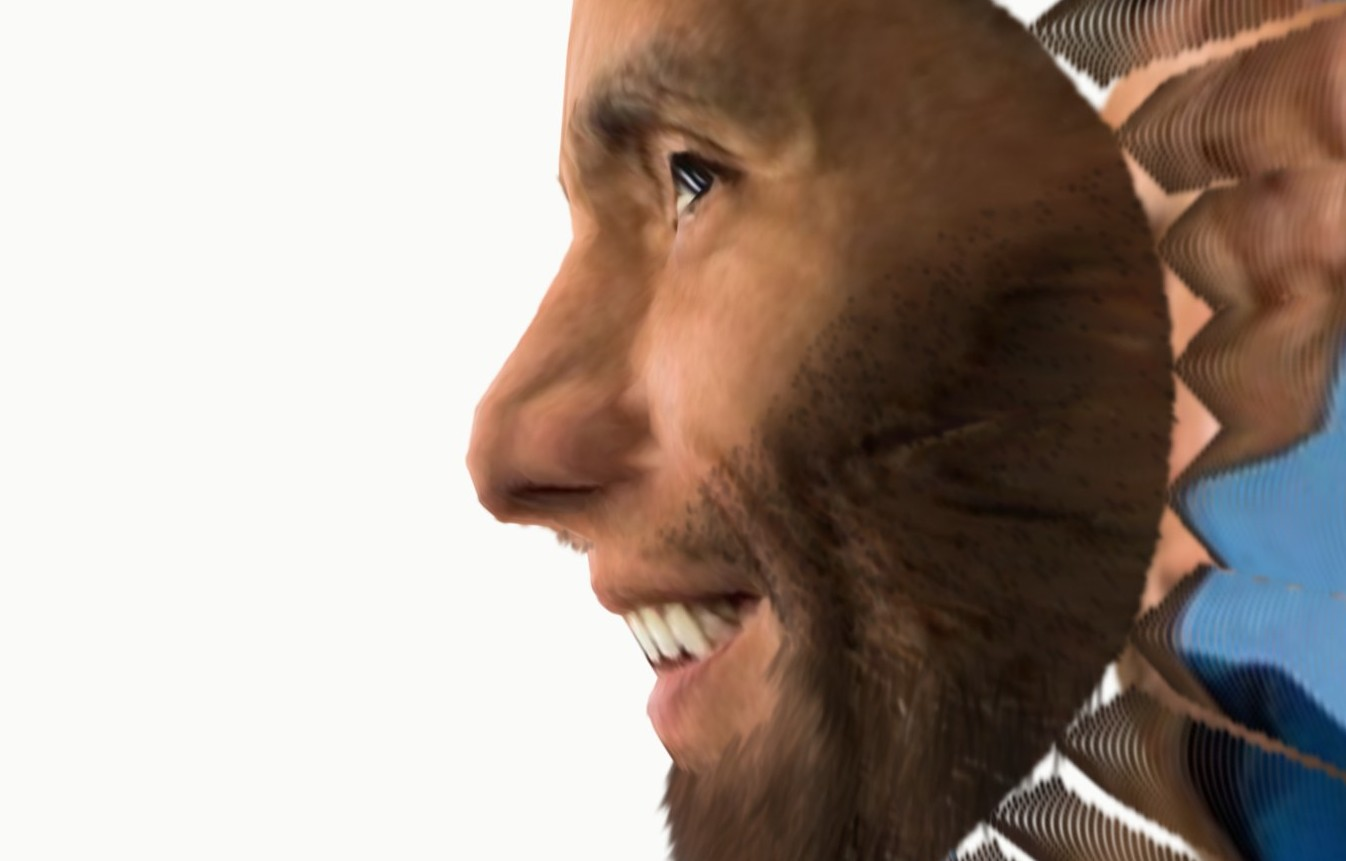
\includegraphics[width=\linewidth]{espejo3d_giro.jpg}\caption{Girada}\end{subfigure}\hfill
  \begin{subfigure}{0.32\linewidth}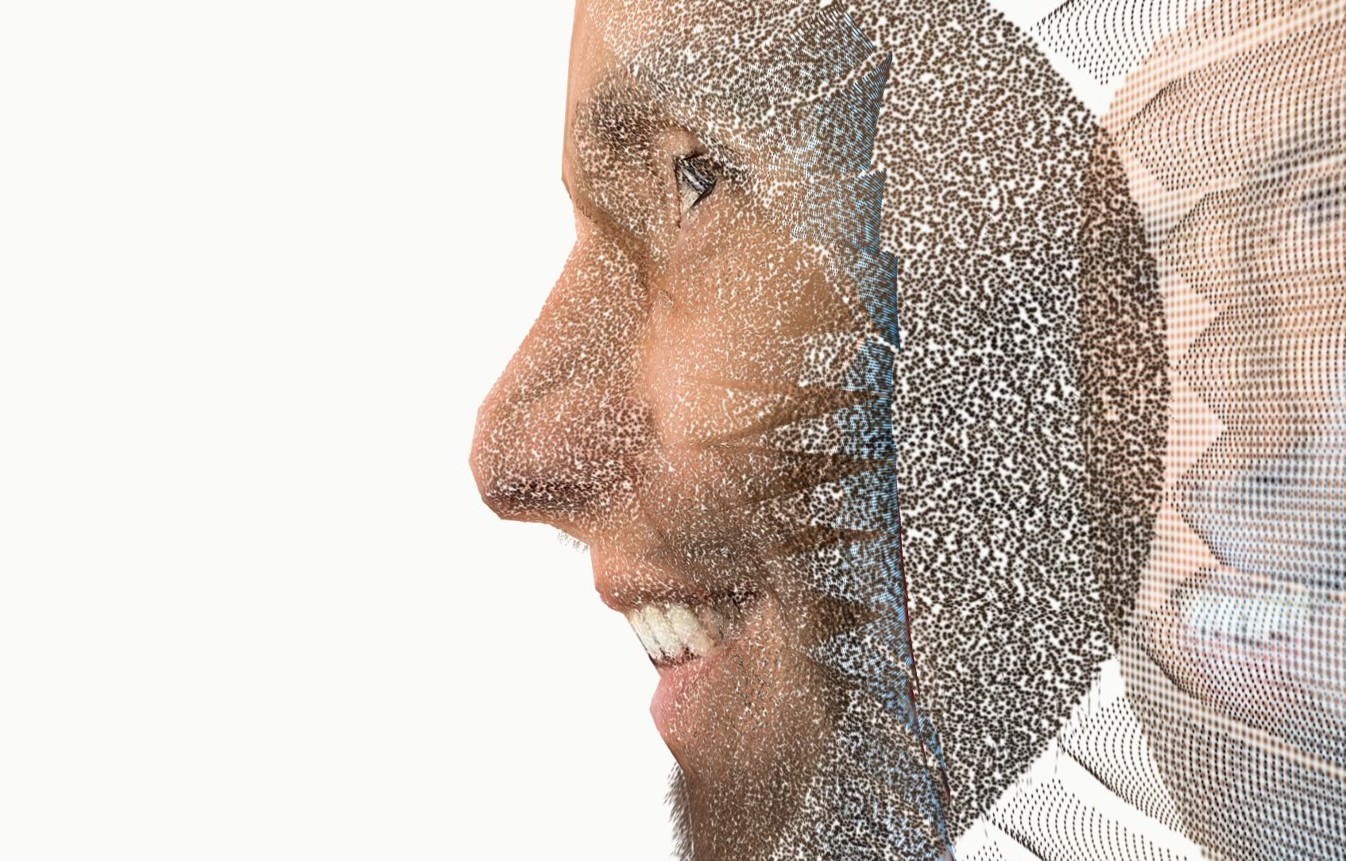
\includegraphics[width=\linewidth]{espejo3d_splats.jpg}\caption{Cada gaussiana}\end{subfigure}
  \caption{Espejo 3D con barba completa, construido desde una sola foto. Al girar mucho se ven los límites de reconstruir desde una vista: el relieve detrás de la cara se estira.}
  \label{fig:espejo}
\end{figure}

\subsection{Peluca 3D multivista}
\label{sec:peluca}

La peluca 3D escanea el peinado de una persona con la cámara y lo convierte en una peluca de gaussianas. Esa peluca se puede ver sobre un maniquí, sobre la cara escaneada o sobre otra persona en vivo (\archivo{splatting/hair3d.py}, \archivo{splatting/face3d.py}, \archivo{compositing/bald.py}).

\textbf{Escaneo.} Durante 12 segundos la persona gira la cabeza unos 180°, y se guardan capturas con el ángulo de giro estimado. En cada captura, la máscara de pelo se obtiene combinando el segmentador, la distancia de color al pelo y una elipse de la cabeza (\archivo{segmentation/transfer_mask.py}).

\textbf{Forma: \emph{visual hull} por cortes.} Para cada altura y cada dirección horizontal (360 direcciones), cada captura indica, desde su ángulo, dónde empieza y dónde termina el pelo. Intersecar esas franjas da el corte transversal real de la peluca, es decir, la envolvente visual \cite{laurentini1994}, calculada rebanada por rebanada. Las direcciones que ninguna captura vio siguen una forma de cabeza:
\begin{itemize}
  \item tan ancha como la vista más frontal;
  \item nunca delante de la cara;
  \item redondeada sobre el cráneo y más plana donde cuelga pelo largo.
\end{itemize}

\textbf{Textura.} Cada punto de la superficie toma color de las capturas que mejor lo ven, mezcladas según qué tan de frente lo ven, para que no haya costuras. La nuca nunca se ve: recibe el color del último pelo que vio cada perfil, con estrías verticales. Cada gaussiana se alarga en la dirección del pelo, estimada con el tensor de estructura (perpendicular al gradiente dominante; hacia abajo donde no hay orientación clara).

\textbf{Estudio.} En el navegador, la peluca se puede editar de tres formas:
\begin{itemize}
  \item \textbf{color}: se recolorean las gaussianas con la intensidad elegida;
  \item \textbf{largo}: se eliminan las gaussianas por debajo de una altura;
  \item \textbf{tijeras}: un pincel en pantalla corta las gaussianas más cercanas a la cámara dentro de su radio, usando la proyección de cada gaussiana; los cortes se pueden deshacer.
\end{itemize}

\textbf{Prueba en vivo.} Para probar la peluca sobre otra persona, el navegador sigue la cabeza con MediaPipe en JavaScript y el servidor quita el pelo propio de esa persona. El fondo se aprende de cuadros anteriores o se rellena, y el cuero cabelludo se sombrea a partir de la piel de la cara. La figura~\ref{fig:peluca} muestra una peluca construida desde una sola foto, el caso mínimo; con el escaneo de 180° se cierra también la parte de atrás.

\begin{figure}[ht]
  \centering
  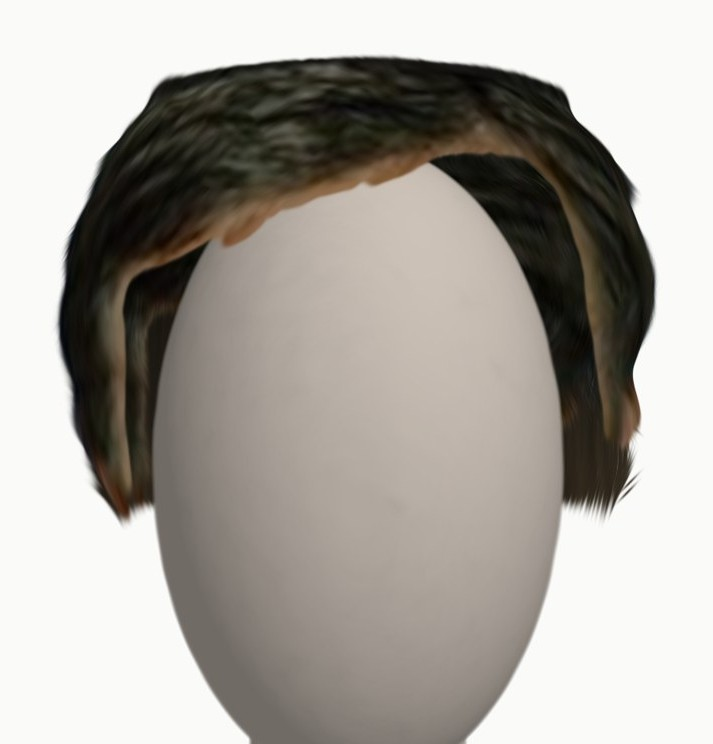
\includegraphics[width=0.55\linewidth]{peluca3d.jpg}
  \caption{Peluca de gaussianas sobre el maniquí, construida desde un único retrato frontal.}
  \label{fig:peluca}
\end{figure}

\subsection{Laboratorio: avatar en vivo}
\label{sec:lab}

El laboratorio (\archivo{lab/avatar.py}) escanea la cabeza desde varios ángulos y construye un avatar de gaussianas. Cada gaussiana guarda su triángulo de la malla, sus coordenadas baricéntricas, un desplazamiento y una covarianza expresados en el marco local del triángulo. Ese marco es ortonormal: $e_1$ es la primera arista normalizada, $n$ la normal y $e_2=n\times e_1$. Con $R=[e_1\;e_2\;n]$ y $s$ el ancho de la cara, la covarianza en el mundo es $R\,\Sigma_{\text{local}}\,R^\top s^2$.

En cada cuadro de la cámara, la malla nueva reconstruye el marco de cada triángulo y la gaussiana lo sigue. Por eso el avatar copia los gestos de la persona y puede verse de perfil. Está marcado como experimental en la interfaz.

\subsection{Contrarreloj: el juego de afeitado}
\label{sec:juego}

La persona tiene 30 segundos para afeitar una barba con física hasta dejar un estilo objetivo: candado, bigote o collar (\archivo{game/speedrun.py}). La ``máquina'' puede ser el mouse o la punta del dedo índice, detectada con el modelo de mano de MediaPipe; corta solo con el índice extendido y el dedo medio doblado.

\textbf{Detección del corte.} A 10~cuadros por segundo, el dedo salta decenas de píxeles entre cuadros, así que probar si toca un punto dejaría pelos sin cortar. En su lugar, se cortan las hebras cuya raíz o primer nodo está a menos de $r=0{,}05\,w$ del segmento recorrido $\overline{p_0p_1}$:
\begin{equation}
  t=\operatorname{clamp}\!\left(\frac{(x-p_0)\cdot(p_1-p_0)}{\lVert p_1-p_0\rVert^2},0,1\right),\qquad d=\lVert x-(p_0+t(p_1-p_0))\rVert.
\end{equation}
Las hebras cortadas caen con física y se desvanecen.

\textbf{Puntaje.} Se calcula como
\begin{equation}
  1000\cdot\text{limpieza}\cdot\text{conservación},
\end{equation}
donde la limpieza es la fracción de pelo afeitado fuera del objetivo y la conservación, la fracción de pelo que queda dentro de él. Se descartó la IoU como puntaje porque, sin tocar nada, ya daba 0{,}72 para el candado.

\begin{figure}[ht]
  \centering
  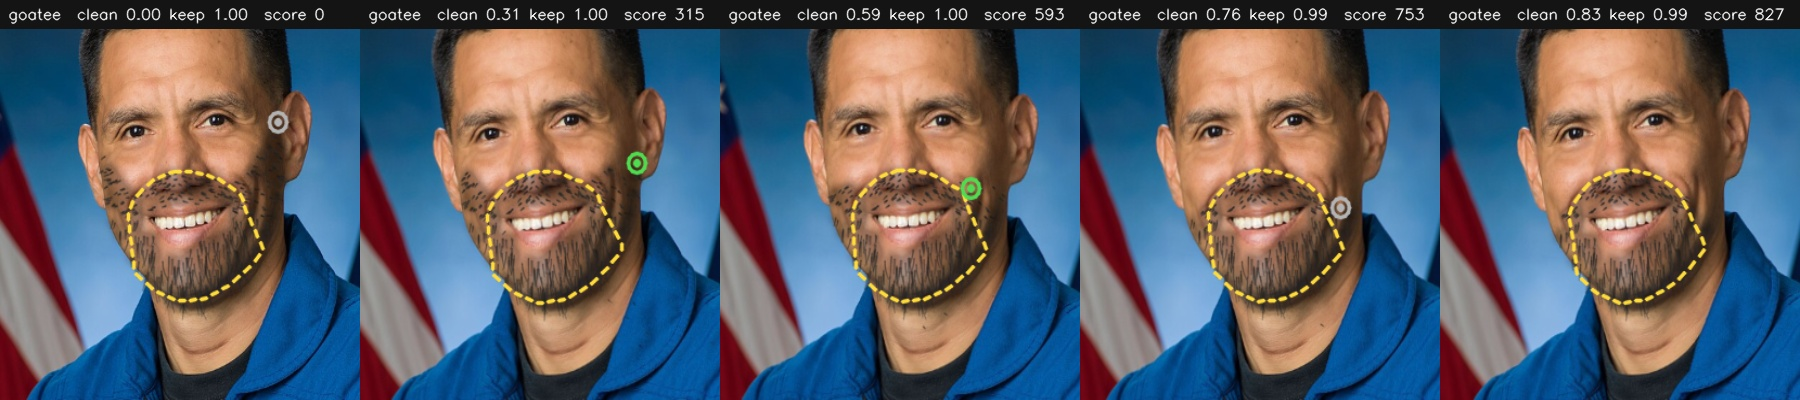
\includegraphics[width=\linewidth]{contrarreloj.jpg}
  \caption{Una ronda de Contrarreloj con objetivo ``candado'', de la barba completa al estilo final.}
  \label{fig:juego}
\end{figure}
